\documentclass[slidestop]{beamer}
\usetheme{JuanLesPins}
\usepackage{fontenc}

\usepackage[english]{babel}
\usepackage[latin1]{inputenc}
\usepackage{times}
\usepackage[T1]{fontenc}
\usepackage{fontenc}
\usepackage{amssymb}
%\usepackage{pgf,pgfarrows,pgfnodes,pgfautomata,pgfheaps}
\usepackage{amsmath,amssymb}
%\usepackage{tikz}
\usepackage{times}
\usepackage{colortbl}

\usebackgroundtemplate{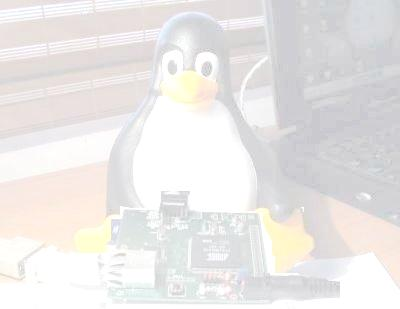
\includegraphics[width=\paperwidth, heigth=\paperheight]{../images/tux_ecb_at91.jpg}}

\title{SIE: Plataforma Hardware \textit{copyleft}  para la Ense�anza de Sistemas Digitales}
\author{Carlos Iv�n Camargo Bare�o}
\institute[Universidad Nacional de Colombia]{Universidad Nacional de Colombia\\
  Departamento de Ingenier�a El�ctrica y Electr�nica}

\pgfdeclareimage[height=.5cm]{logo}{../images/logo_unal}
\logo{\pgfuseimage{logo}}



\begin{document}

%----------------------------------------------------------------------INSERT TITLE-
\frame[c]{\titlepage}
\frame[c]{\tableofcontents}

%$$$$$$$$$$$$$$$$$$$$$$$$$$$$$$$$$$$$$$$$$$$$$$$$$$$$$$$$$$$$$$$$$$$$$$$$$$$$$$$$$$$
%----------------------------------------------------------------------Introducci�n-
\section{Sistemas Embebidos}
%$$$$$$$$$$$$$$$$$$$$$$$$$$$$$$$$$$$$$$$$$$$$$$$$$$$$$$$$$$$$$$$$$$$$$$$$$$$$$$$$$$$

\subsection[Embedded]{Aplicaciones}


\begin{frame}
  \frametitle{Sistemas Embebidos: Aplicaciones}
   \begin{center} 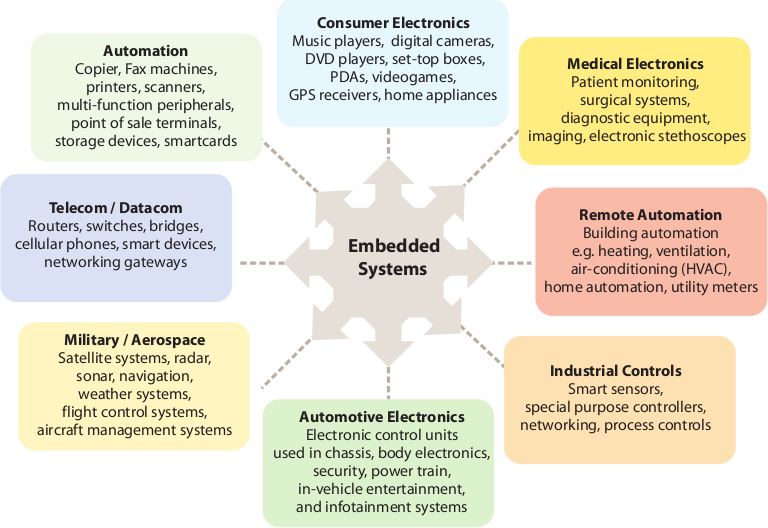
\includegraphics[scale=.5]{../images/Embedded_systems_applications.png}   \end{center}
\end{frame}


\subsection[Embedded]{Arquitectura}

\begin{frame}
  \frametitle{Sistemas Embebidos: Arquitectura}
   \begin{center} 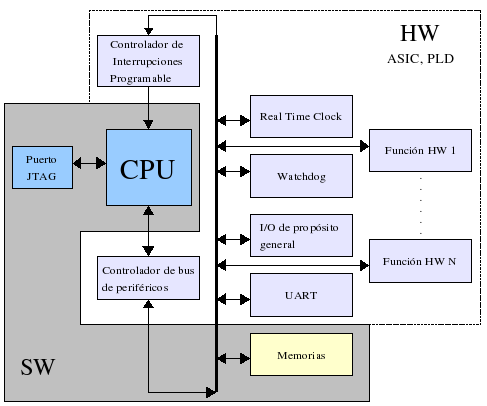
\includegraphics[scale=.5]{../images/ES_Architecture.png}   \end{center}
\end{frame}


\subsection[Embedded]{Conocimientos Necesarios}
\begin{frame}
  \frametitle{Sistemas Embebidos: Aplicaciones}
   \begin{center} 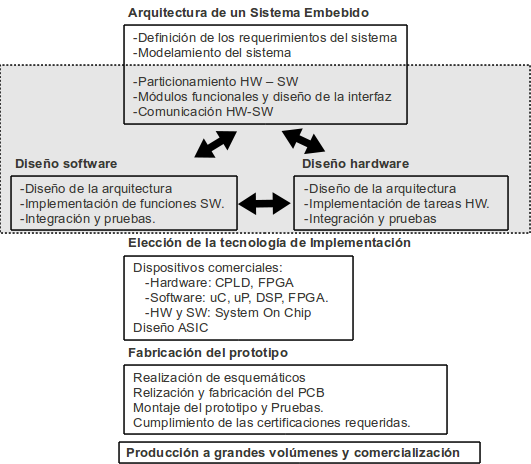
\includegraphics[scale=.51]{../images/ES_CDIO_flow.png}   \end{center}
\end{frame}



%$$$$$$$$$$$$$$$$$$$$$$$$$$$$$$$$$$$$$$$$$$$$$$$$$$$$$$$$$$$$$$$$$$$$$$$$$$$$$$$$$$$
%----------------------------------------------------------Metodolog�a de Ense�anza-
\section{Metodolog�a de Ense�anza}
%$$$$$$$$$$$$$$$$$$$$$$$$$$$$$$$$$$$$$$$$$$$$$$$$$$$$$$$$$$$$$$$$$$$$$$$$$$$$$$$$$$$

\begin{frame}
  \frametitle{Divisi�n implementada en la Universidad Nacional de Colombia}
 \begin{figure}[htpb]
   \begin{center} 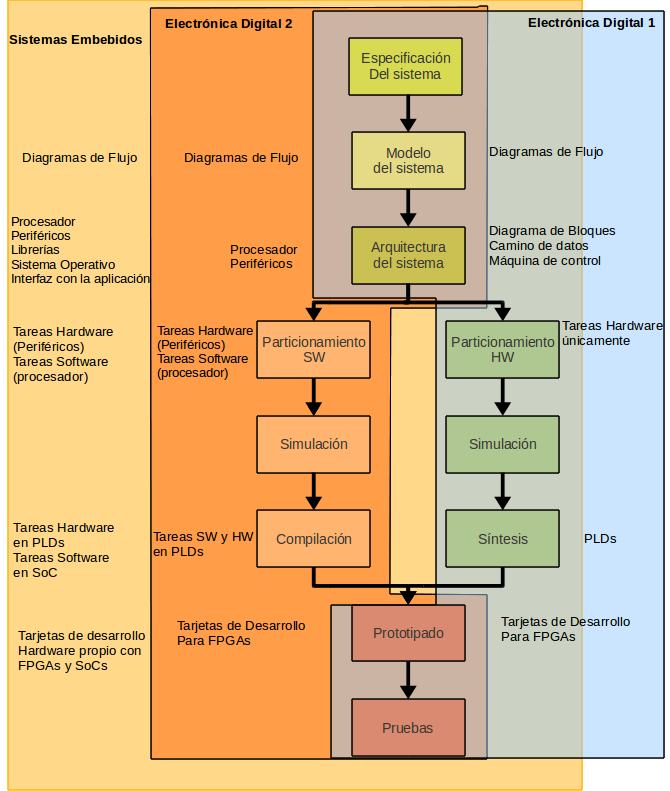
\includegraphics[scale=.33]{../images/habilidades_digitales.png}   \end{center}
 \end{figure}
\end{frame}

%$$$$$$$$$$$$$$$$$$$$$$$$$$$$$$$$$$$$$$$$$$$$$$$$$$$$$$$$$$$$$$$$$$$$$$$$$$$$$$$$$$$
%----------------------------------------------------------Metodolog�a de Ense�anza-
\section{Plataforma Copyleft Hardware SIE}
%$$$$$$$$$$$$$$$$$$$$$$$$$$$$$$$$$$$$$$$$$$$$$$$$$$$$$$$$$$$$$$$$$$$$$$$$$$$$$$$$$$$

\subsection{Especificaciones}

\begin{frame}
  \frametitle{SIE: Especificaciones}
 \begin{figure}[htpb]
   \begin{center} 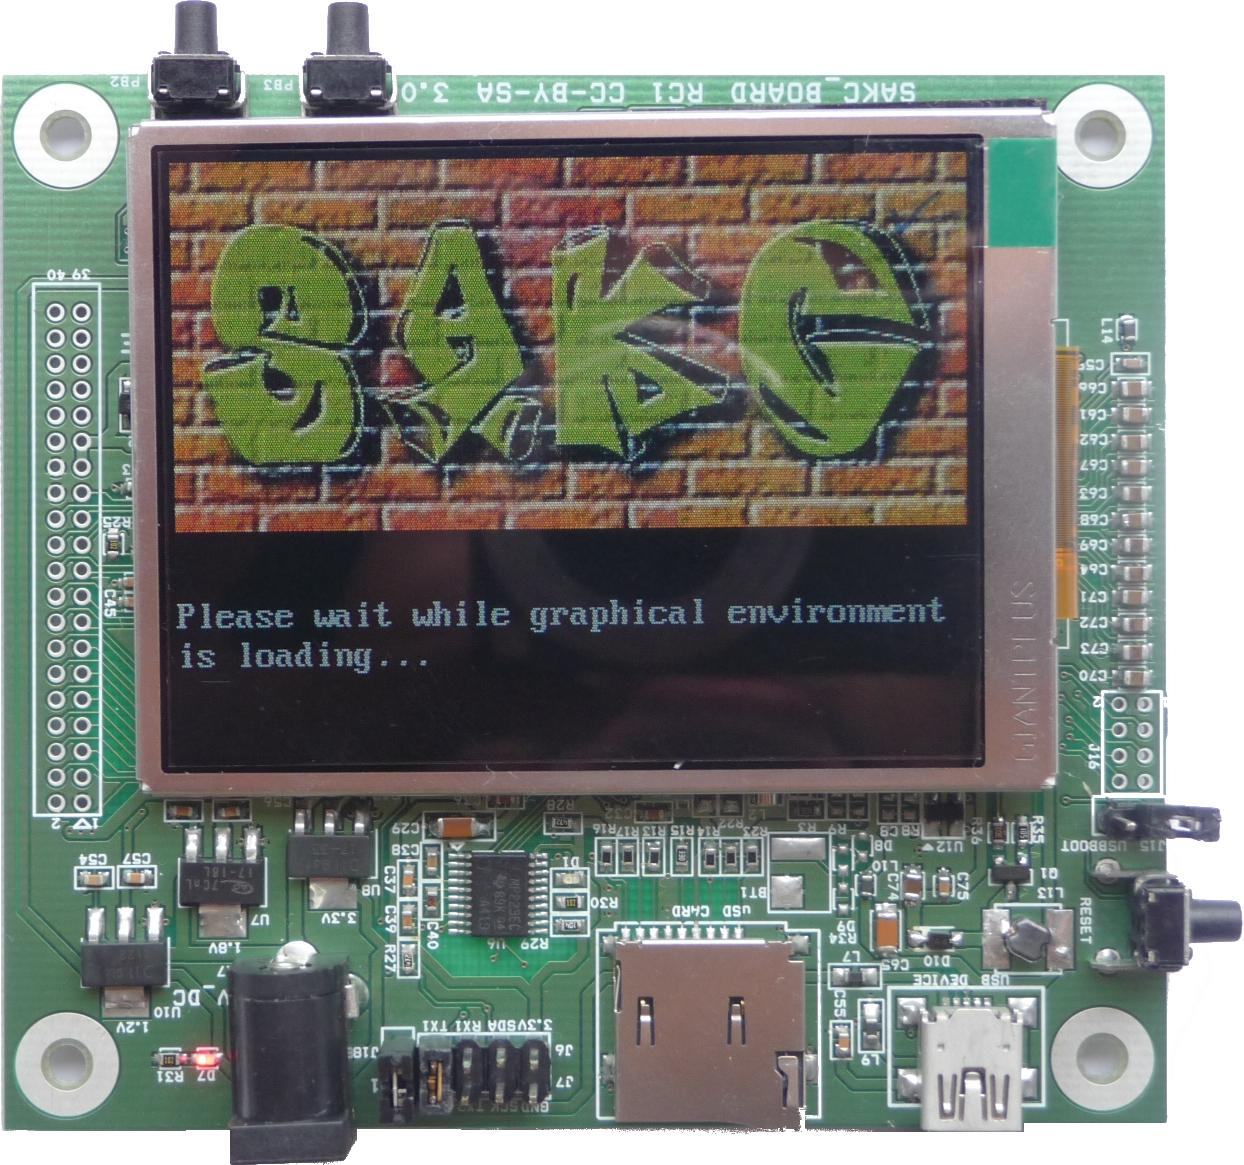
\includegraphics[scale=.5]{../images/SIE.jpg}   \end{center}
 \end{figure}
\end{frame}

\subsection{Diagrama de Bloques}

\begin{frame}
  \frametitle{SIE: Diagrama de Bloques}
 \begin{figure}[htpb]
   \begin{center} 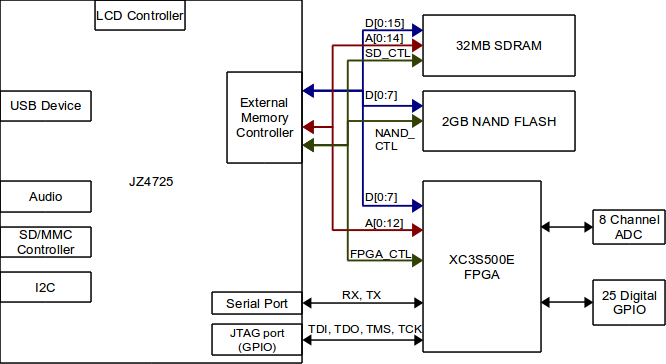
\includegraphics[scale=.5]{../images/SIE_block_diagram.png}   \end{center}
 \end{figure}
\end{frame}

\subsection{SIE: Plataforma hardware copyleft }
 
 \begin{frame}

  \frametitle{SIE: Plataforma hardware copyleft}

     \begin{block}{ }
      \begin{itemize}
       \item Acceso a los archivos de dise�o realizados en herramientas abiertas (kicad en este caso)
       \item Posibilidad de hacer cambios f�sicos y funcionales.
       \item Acceso a notas de aplicaci�n, dise�os de referencia.
       \item Acceso al software b�sico: \textit{bootloader} \textit{kernel} \textit{sistema de archivos}
       \item Soporte a trav�s de listas de discusi�n.
       \item Acceso a los fabricantes de las tarjetas.
      \end{itemize}
     \end{block}

    \begin{alertblock}{}
      Todo esto puede descargarse de: http://wiki.linuxencaja.net/wiki/GIT
    \end{alertblock}

 \end{frame}

 \begin{frame}


     \begin{alertblock}{Licencia: Creative Commons BY - SA}
      \textbf{BY} Permite distribuir, modificar y construir sobre su trabajo, incluso con fines comerciales, siempre y cuando se de cr�dito a la creaci�n original.                                   \\
      \textbf{BY - SA}: Todo trabajo derivado debe tener la misma licencia.
     \end{alertblock}


 
 \end{frame}



%$$$$$$$$$$$$$$$$$$$$$$$$$$$$$$$$$$$$$$$$$$$$$$$$$$$$$$$$$$$$$$$$$$$$$$$$$$$$$$$$$$$
%----------------------------------------------------------Metodolog�a de Ense�anza-
\section{SIE en la Ense�anza de Dise�o Digital}
%$$$$$$$$$$$$$$$$$$$$$$$$$$$$$$$$$$$$$$$$$$$$$$$$$$$$$$$$$$$$$$$$$$$$$$$$$$$$$$$$$$$

\begin{frame}
  \frametitle{SIE en el curso b�sico de digitales}
   \begin{center} 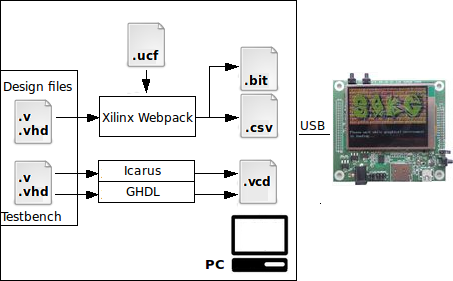
\includegraphics[scale=.75]{../images/HW_design_flow.png}   \end{center}
\end{frame}

\begin{frame}
 \begin{figure}[htpb]
  \frametitle{SIE en el curso b�sico de Arquitectura de Computadores}
   \begin{center} 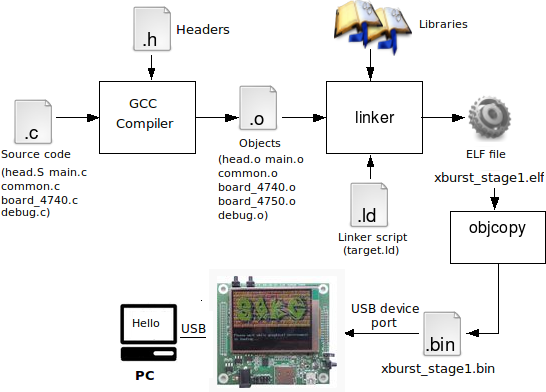
\includegraphics[scale=.55]{../images/SW_design_flow.png}   \end{center}
 \end{figure}
\end{frame}


\begin{frame}
  \frametitle{Interfaz HW/SW de SIE}
   \begin{center} 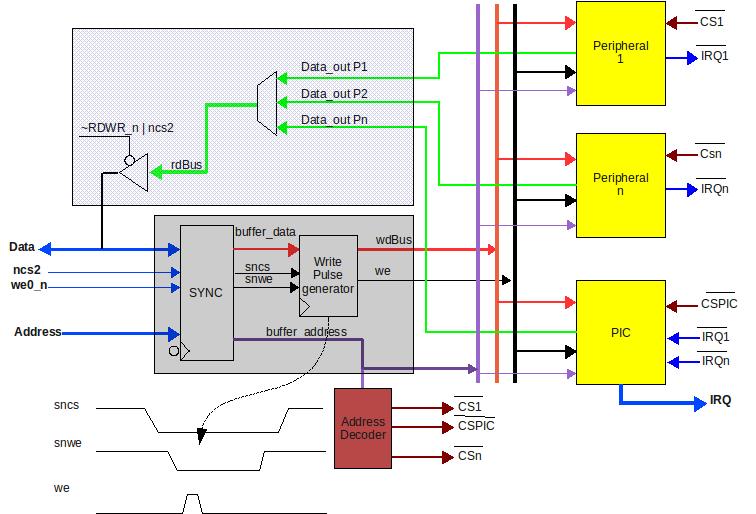
\includegraphics[scale=.45]{../images/Sw_hw_fpga_arch.png}   \end{center}
\end{frame}


\begin{frame}
  \frametitle{SIE en el curso Sistemas Embebidos}
   \begin{center} 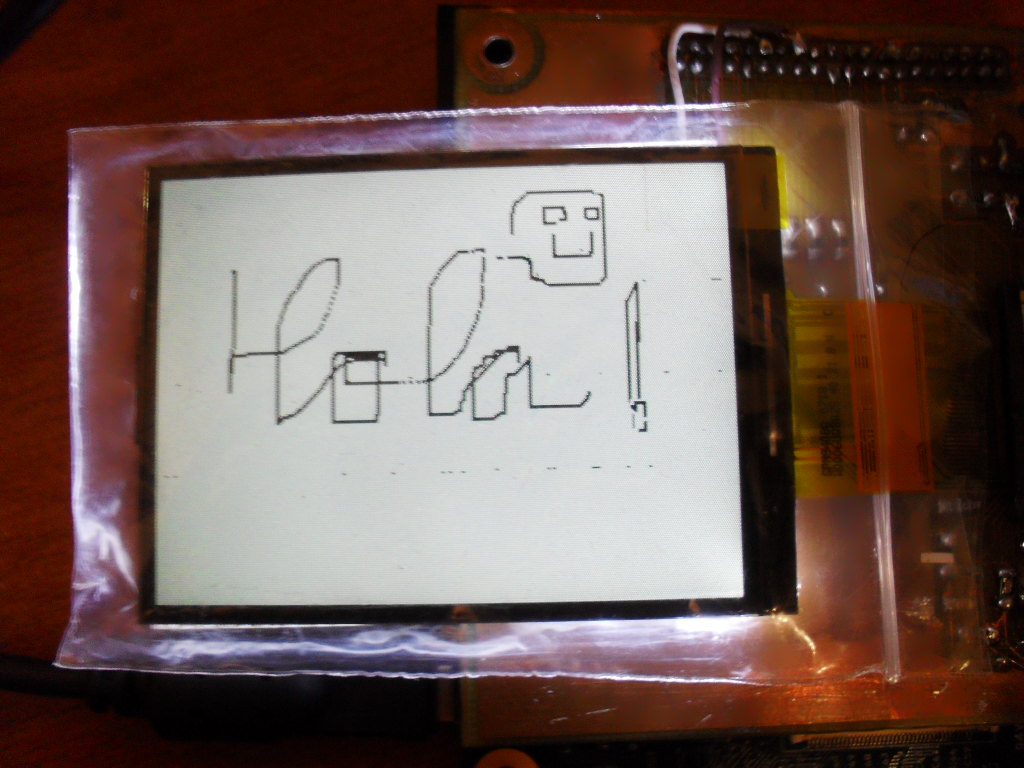
\includegraphics[scale=.15]{../images/Academic_Paint.JPG}   
                  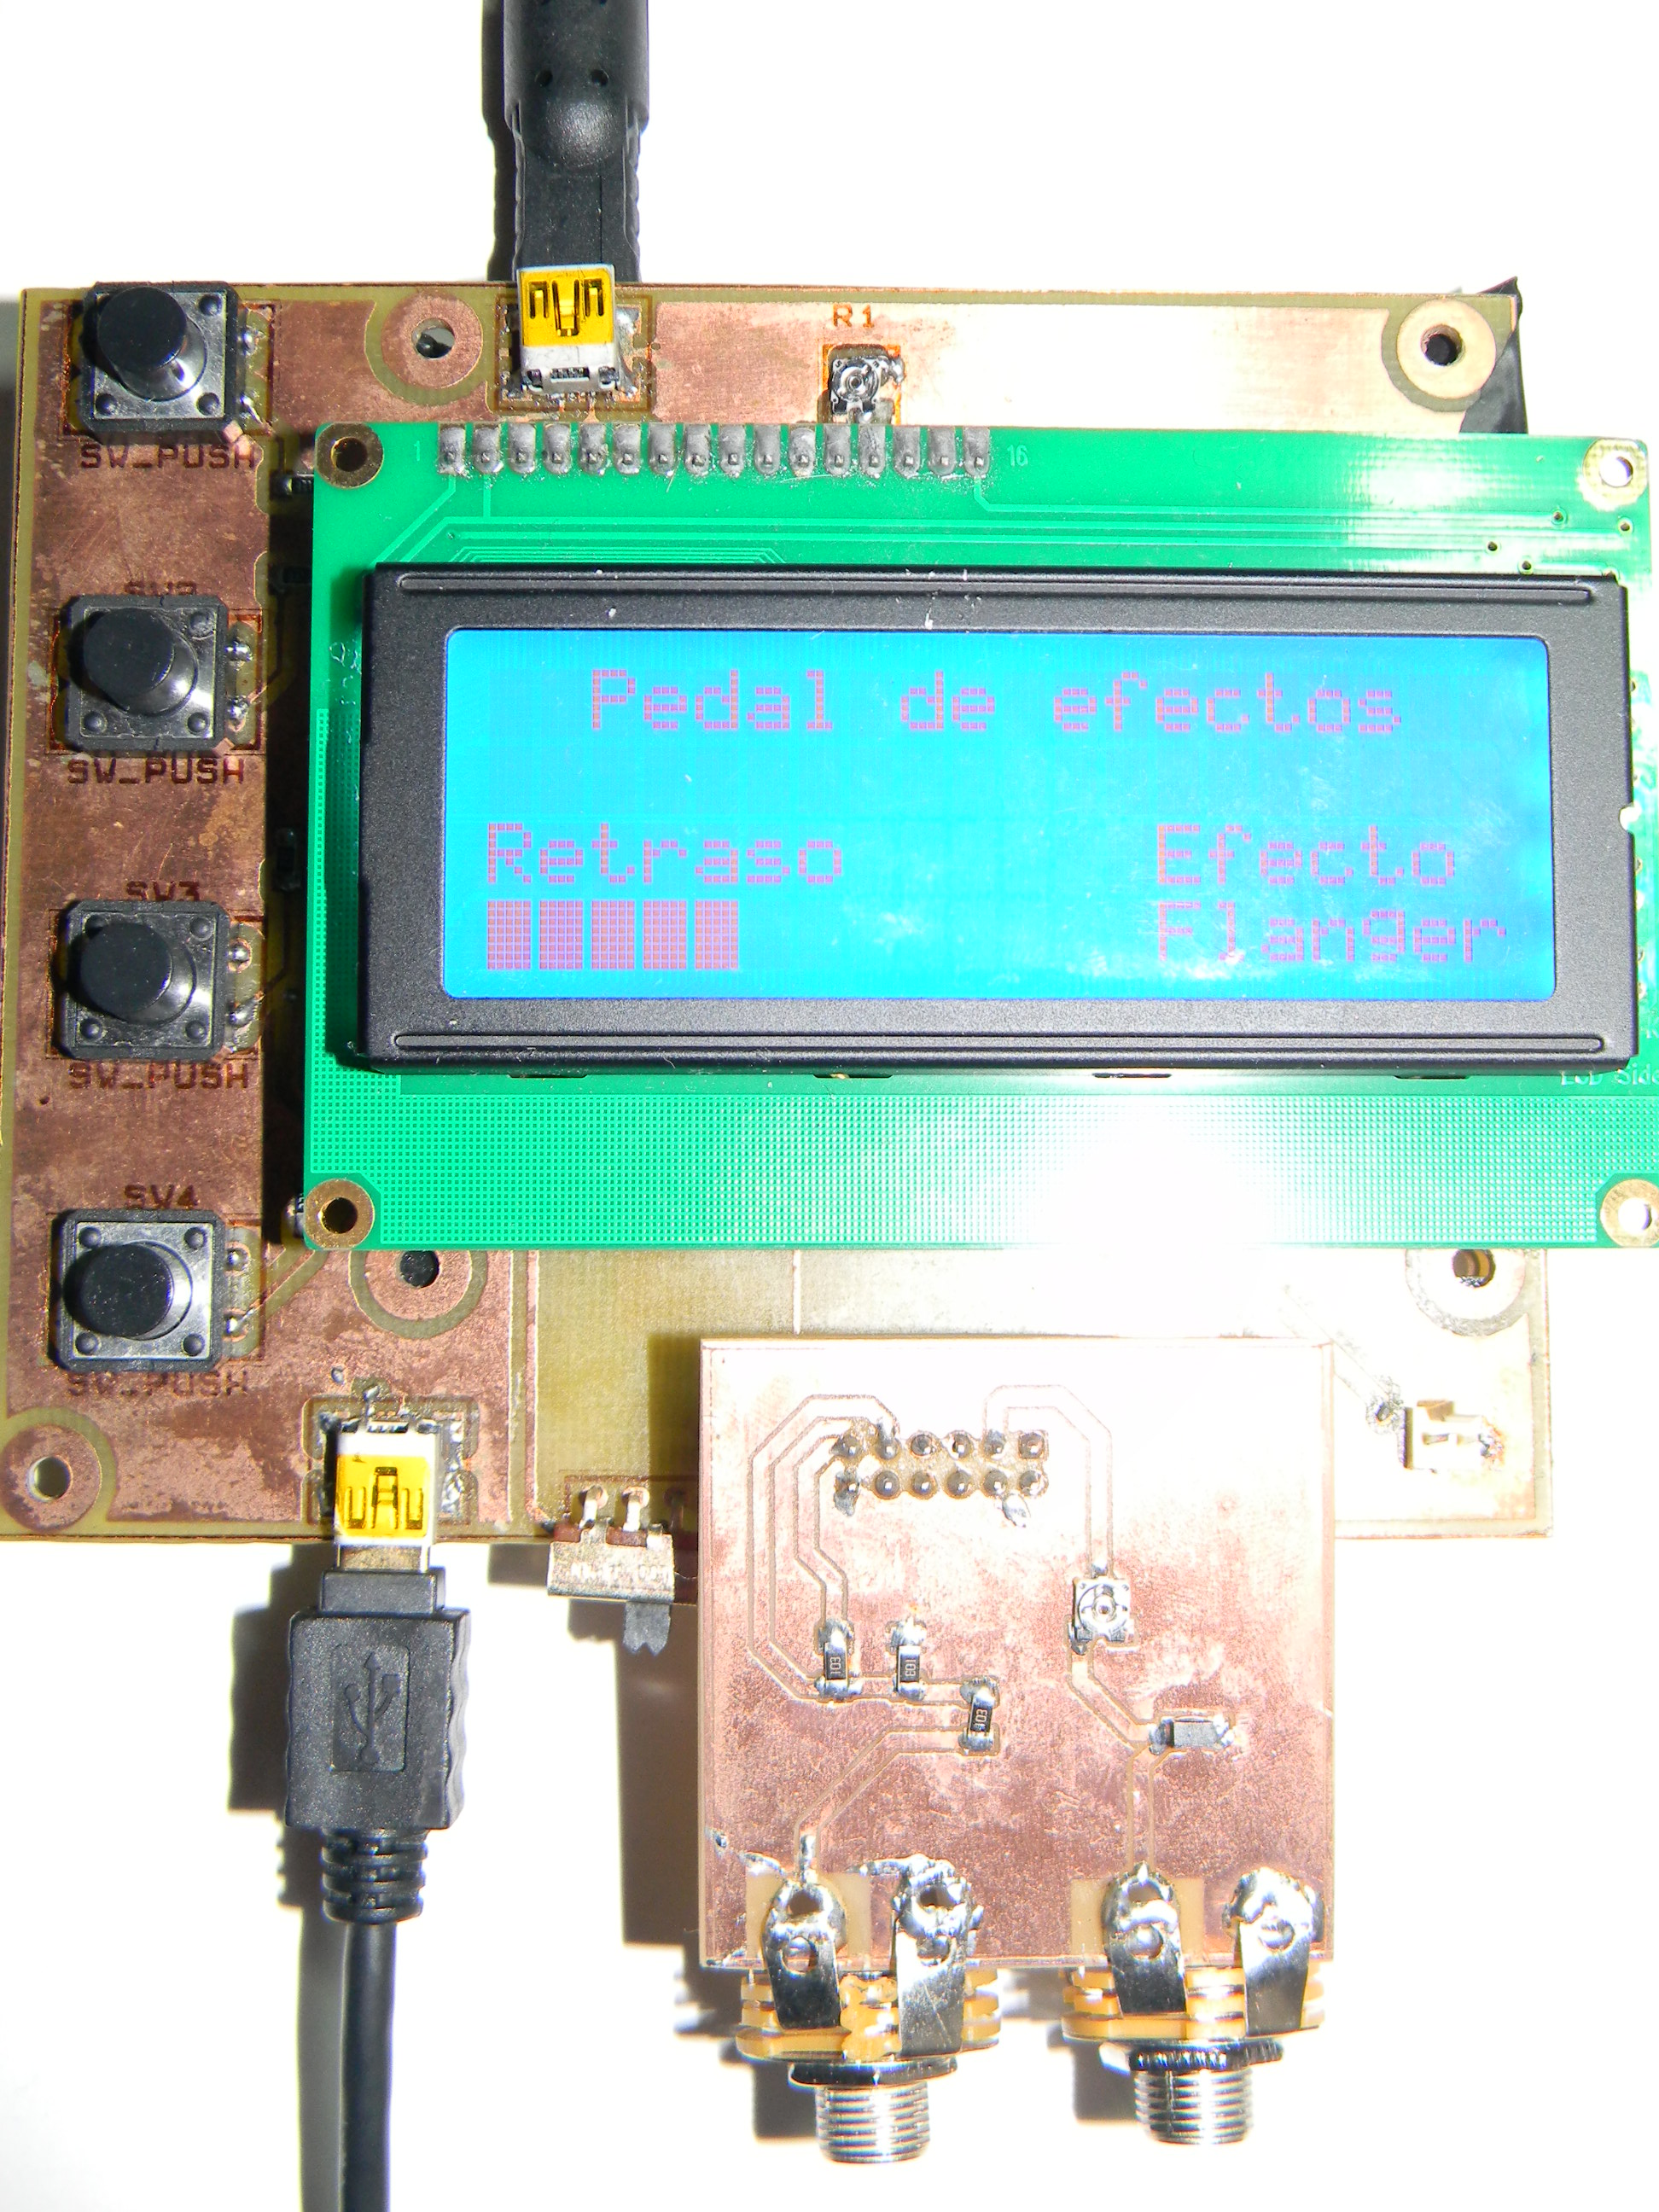
\includegraphics[scale=.05]{../images/Academic_Pedal.JPG}   \\
                  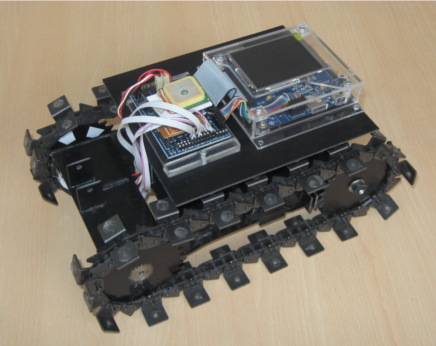
\includegraphics[scale=.3]{../images/Academic_Siebot.png}   
                  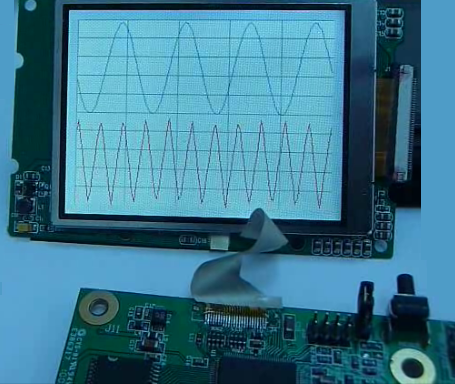
\includegraphics[scale=.35]{../images/Academic_Scop.png}   
   \end{center} 


\end{frame}

 
 \begin{frame}
   \begin{center}
\includegraphics[scale=.15]{../images/gracias}
   \newline
   \huge{�Gracias!}
   \end{center}
 \end{frame}

\end{document}
